%!TEX root=../main.tex

\appendix

\section{Effect of Index of Corrupted Query}
\label{app:qidx}

A key parameter for our experiments is the location of the corrupted query ($idx$).  
\alex{Have we discussed anywhere yet that we focus on single errors?}
This parameter determines the number of queries \sys must consider when searching for a fix,
and affects the size of the complaint set.  
\alex{It won't be clear to the reader how this relates to the size of the complaint set.}
Both of these characteristics directly impact \sys's 
runtime performance. For this reason, it is undesirable to randomly pick and corrupt queries
throughout the query log, as the performance and accuracy results may not be comparable. 
To better understand the relationship between $idx$ and the size of the complaint set, we ran
simulations using a database with $20$ attributes, and a query log of size $1000$ containing
either all $set = const$ or $set = rel$ \texttt{UPDATE} queries.
We varied  $idx$ uniformly throughout the query log, and additionally varied
the skew $s$ and range $r$ parameters to study how they affect the size of the complaint sets.


  \begin{figure}[h]
  \centering
  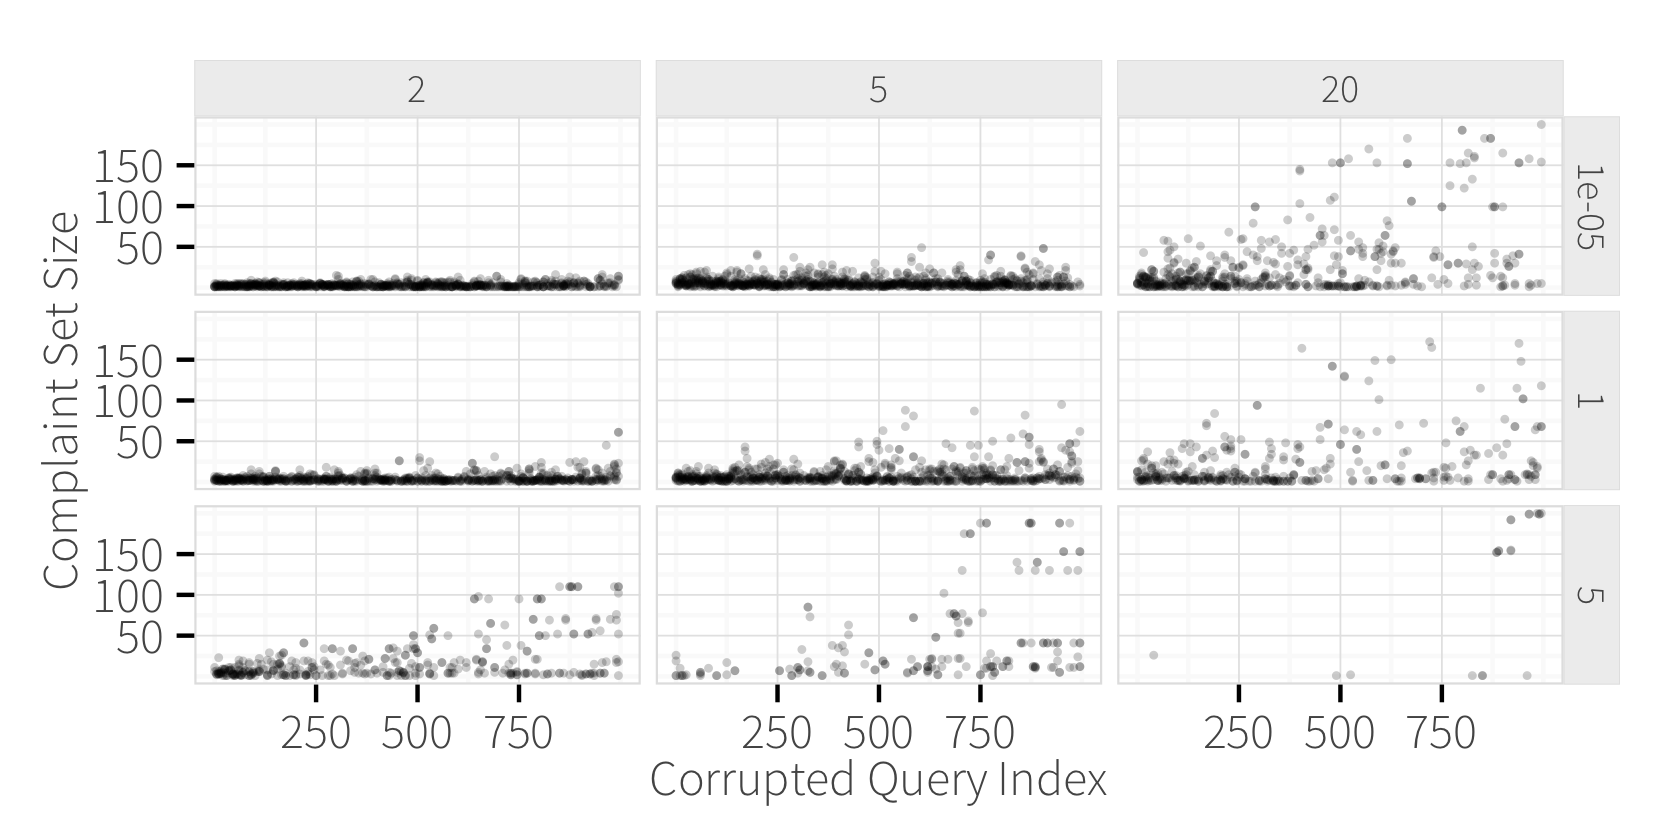
\includegraphics[width = 3.5in]{figures/qidxsimulation/qidx_v_ncomplaints_20attrs_const}
  \caption{Query index vs complaint set size for $set = const$.}
  \label{f:qidx_v_ncomplaints_const} 
  \end{figure}


Figure~\ref{f:qidx_v_ncomplaints_const} plots a representative set of parameters.  We plot one point
for each corrupted query index that results in a complaint set with at least one complaint. 
These results highlight several interesting trends.  When queries do not overlap ($r = 1$, leftmost column),
the size of the complaint sets are relatively small, and their frequency is constant across the possible query indices.
However as the possibility of overlap increases (e.g., $r$ increases), more recent queries are more likely to result in
very large complaint sets (at times the size of the database).   
This effect is a symptom of the fact that queries with large ranges will set groups of tuples to the same value,
and over time, skew the distribution of tuple values to a small number of possible values.
Thus, more recent corruptions that affect a large cluster of similar tuples will result in a large complaint set.
We find that increasing the skew parameter also exacerbates this effect.  
In addition, high skew increases the likelihood that queries will share the same \texttt{WHERE} and \texttt{SET} clause 
attributes as a corrupted query, thus overwriting the error introduced by the corrupted query.  
This is why the frequency of non-empty complaint sets decreases significantly as $s$ increases.


\begin{figure}[h]
\centering
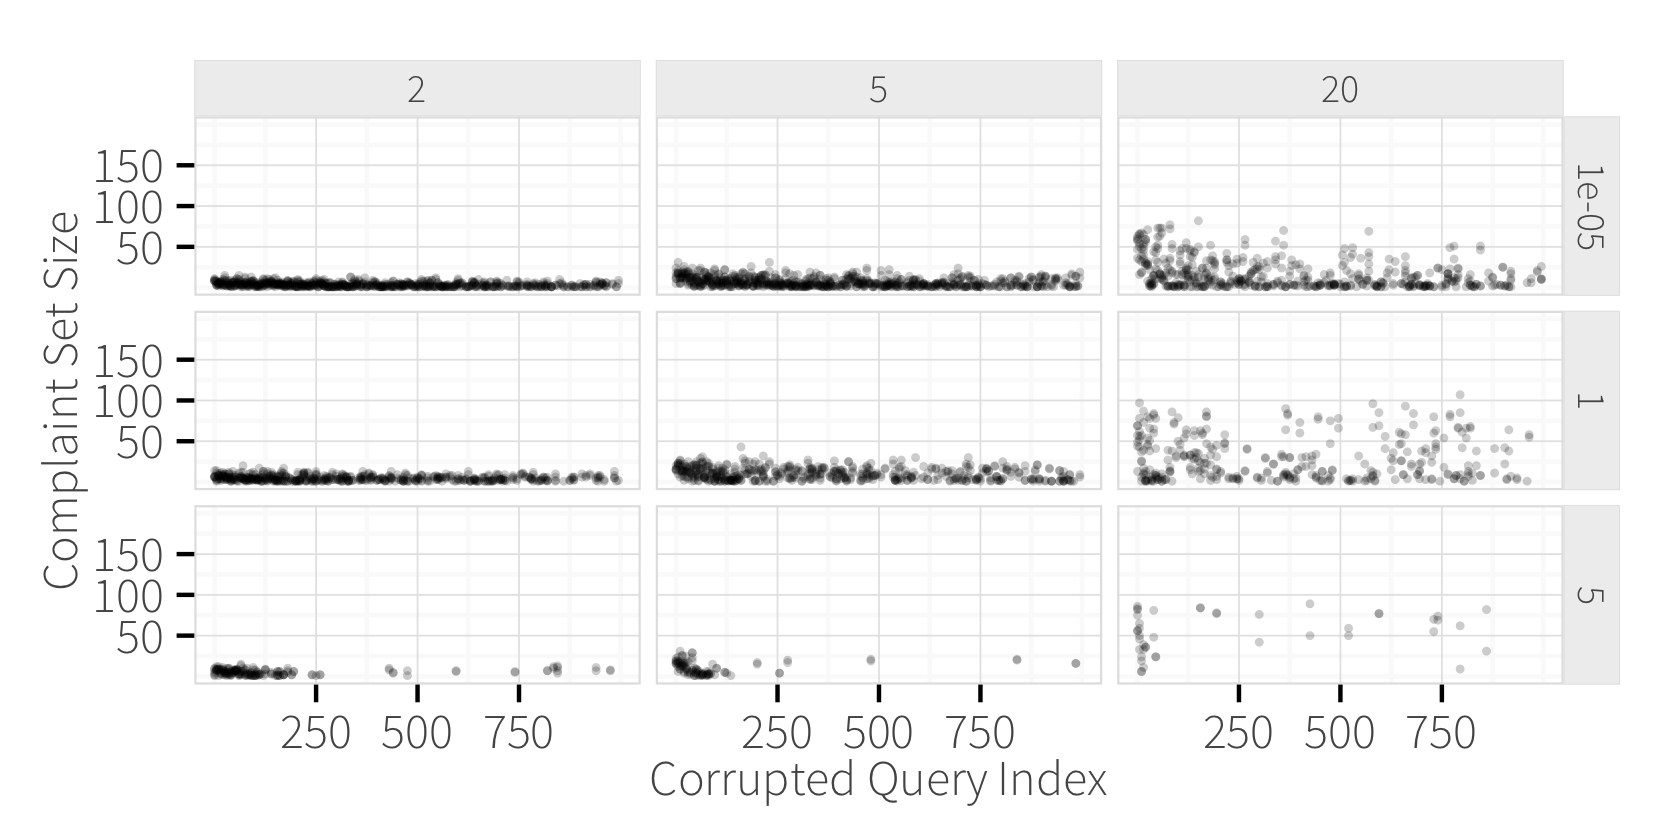
\includegraphics[width = 3.5in]{figures/qidxsimulation/qidx_v_ncomplaints_20attrs_rel}
\caption{Query index vs complaint set size for $set = rel$.}
\label{f:qidx_v_ncomplaints_rel} 
\end{figure}

In contrast to $set=const$ queries, Figure~\ref{f:qidx_v_ncomplaints_rel} executes the 
same experiment using $set=rel$ queries.  In this setting, we find that the trend is
reversed, and older corruptions tend to result in larger complaint sets.  This is because,
subsequent \texttt{UPDATE} queries increment or decrement the attribute value, rather than
overwriting it with a constant value.  The clustering of data values due to query overlap
then increases the number of other tuples affected.


\ewu{summarize findings and implications to experiments here.}
not all corruptions result in complaint sets.
In constant SET clause workloads, larger complaints sets are more likely to
result from more recent corrupted queries -- particularly if the queries are range updates or
the updated attributes are skewed.
For this reason, our experiments corrupt the query log at six positions 
$idx \in \{0, 25, 50, 100, 200, 250\}$ , relative 
to the most recent query (e.g., the most recent query, the $25^th$ most recent query, and so on).

% \begin{figure}[h]
% \centering
% 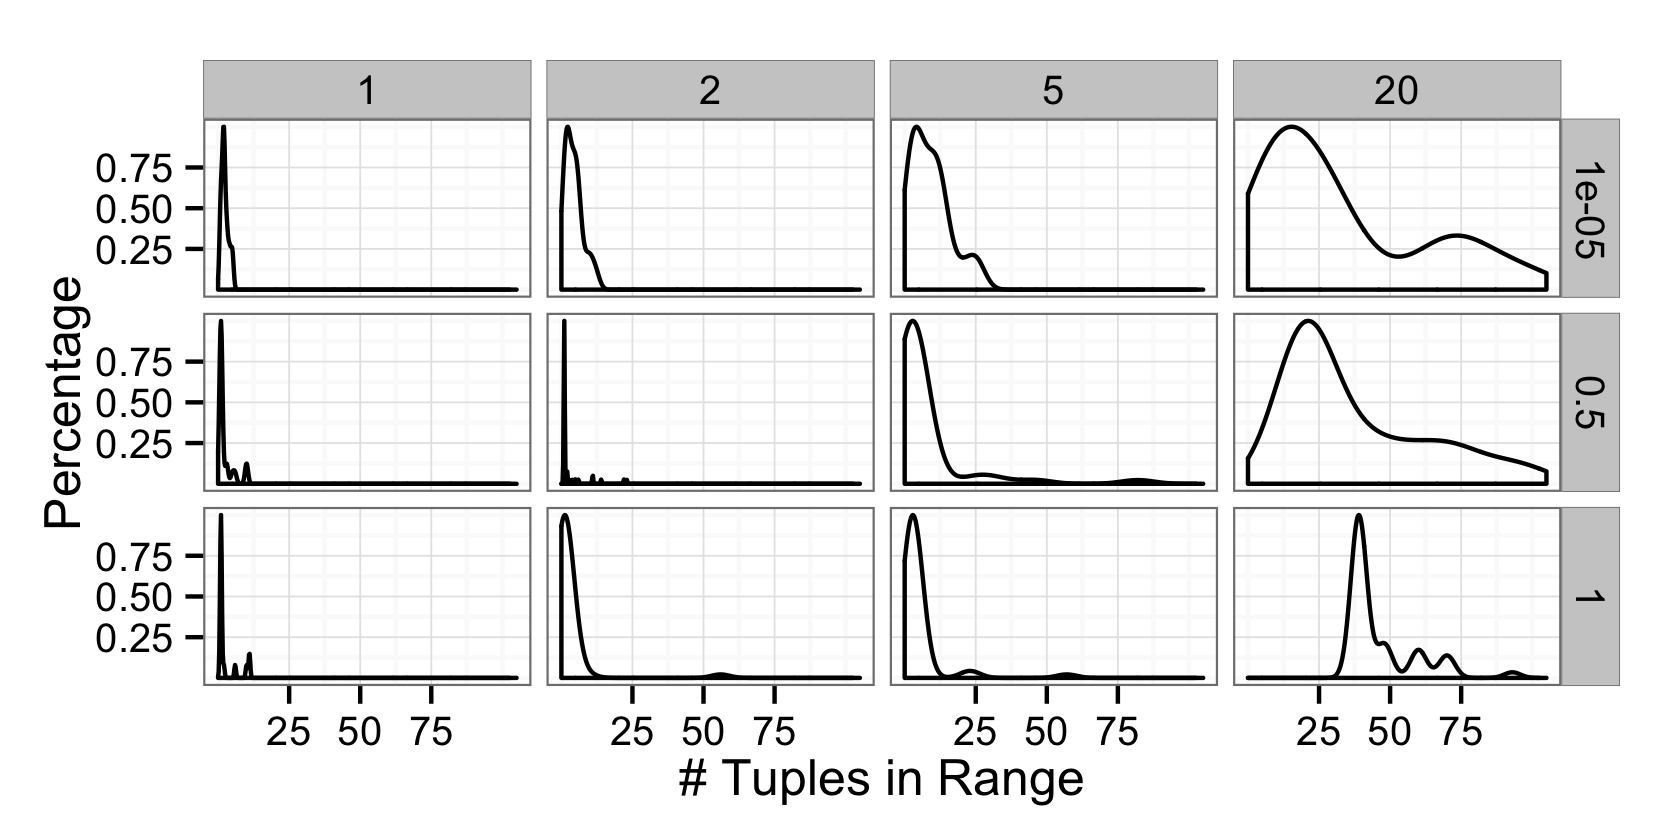
\includegraphics[width = 3.5in]{figures/qidxsimulation/numinrange}
% \caption{.}
% \label{f:numinrange} 
% \end{figure}


As we observed from Figure~\ref{f:multiquery}, \milpall maintains high accuracy when errors
happen more recent, however it does not scale when the error locate further from the most
recent query. \milptuple scales better than \milpall, but ignoring tuples not 
in the complaint set apparently hurts the precision. \milptuplestopearly run times faster
than \milpall and \milptuple, however the aggressive strategy greatly reduce the 
precision. In the end, \milpadvtuple significantly improves the precision with very limited
time cost compare to \milptuple. \\
Based on these observations, we only include the performance of \milpadvtuple and \milpadvall
in the rest of the experiments. 


\section{Heuristic Approaches}
In this section, we compare \heurstic and \milpall on query log with size 1. 
We use \textbf{Synthetic} data generator (Section~\ref{sec:syntheticgen}) 
to generate a initial table with 1000 tuples and one 
\texttt{UPDATE} query with range update. 
We further adjust the range (\# of tuples modified by the query) 
from 5 tuples to 500 tuples. 



  \begin{figure}[h]
  \centering
    \begin{subfigure}[t]{.23\textwidth}
    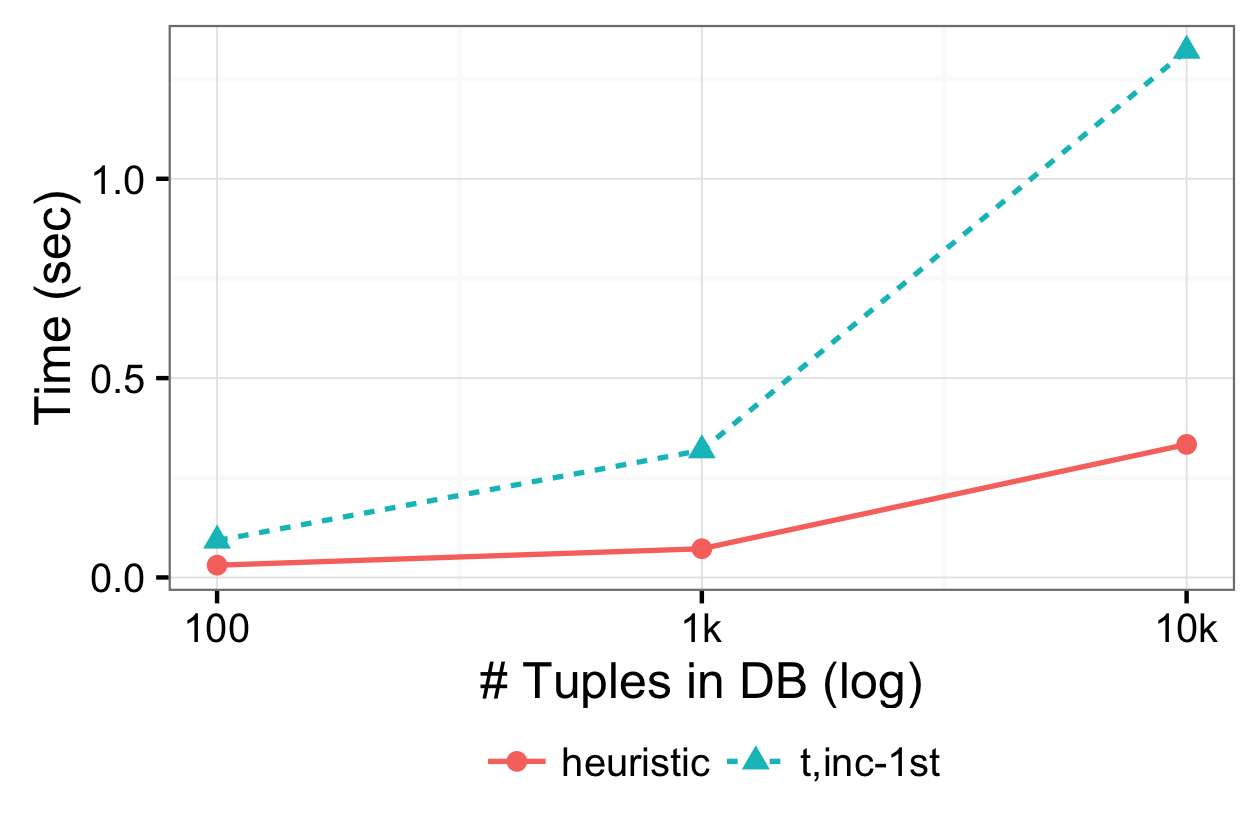
\includegraphics[width = .9\columnwidth]{figures/heuristictime}
    \vspace*{-.1in}
    \caption{Performance of Heuristic Approach vs. \sys.}
    \label{f:heuristic_time} 
    \end{subfigure}
    \begin{subfigure}[t]{.23\textwidth}
    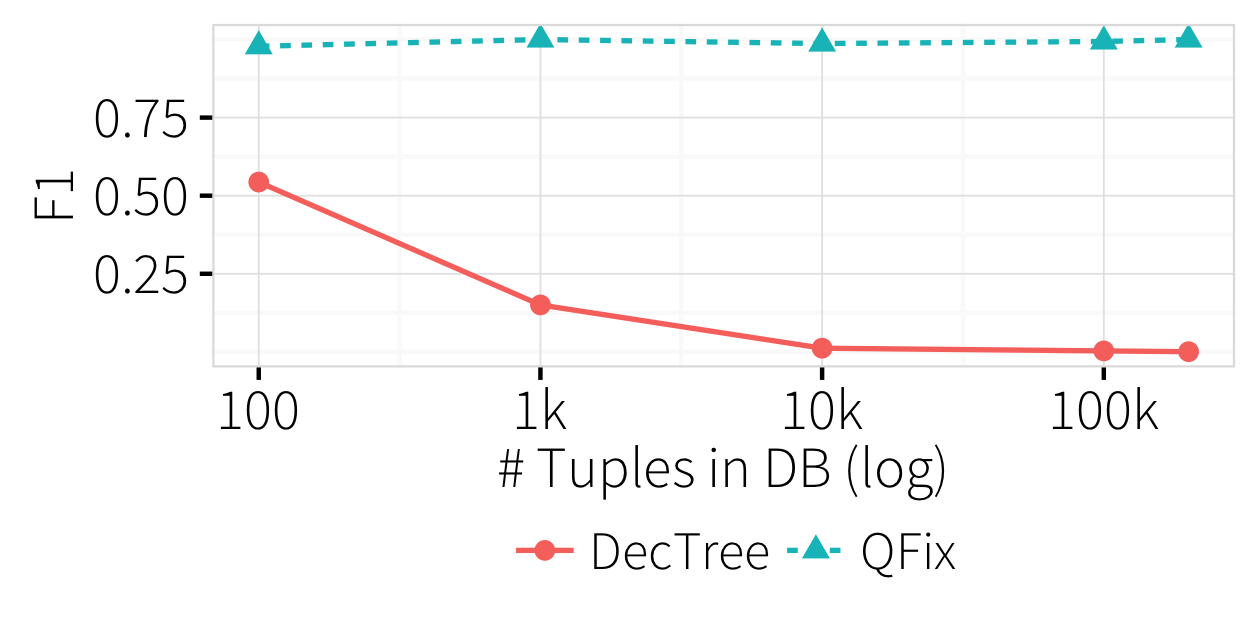
\includegraphics[width = .9\columnwidth]{figures/heuristicacc}
    \vspace*{-.1in}
    \caption{Accuracy of Heuristic Approach vs. \sys.}
    \label{f:heuristic_acc} 
    \end{subfigure}
    \vspace*{-.1in}
    \caption{Heuristic Approach vs. \sys on Single-Query. }
  \end{figure}
  
